\chapter*{Engineering 98}
\addcontentsline{toc}{chapter}{Engineering 98}

\begin{center}
    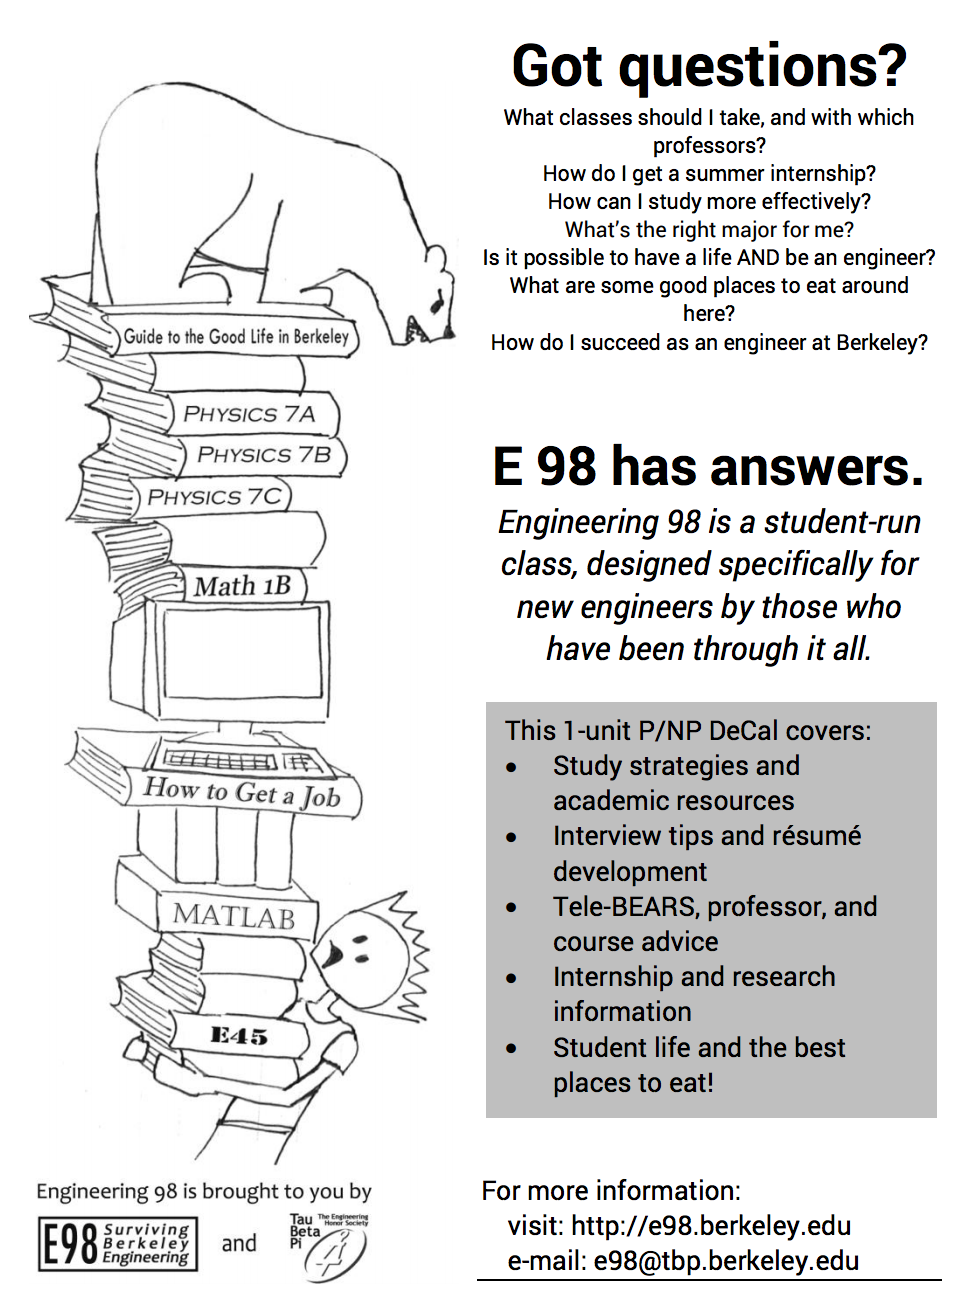
\includegraphics[width=0.9\textwidth]{resources/e98-flyer.png}
\end{center}

\newpage
\chapter*{Engineering 98/198: Spring Edition}
On top of the E98 course offered in the Fall to help students get oriented, the Engineering Science (ES) department offers a seminar course in the Spring that can be very valuable to ES students unsure about how to navigate Berkeley's world of research.
 
ENGIN 98/198 is a seminar series in which you will learn about the research that's taking place right here at Cal by engineering faculty. Guest speakers will discuss their current research and how you can develop your interests into opportunities.  Professor Arias, a faculty advisor for the Engineering Science department, is the organizer for this course, and she makes sure to pull speakers from a broad range of fields. This course is offered Pass/No Pass for 1 credit. 90\% attendance is required for a Pass, but there are no other requirements.  Engineering Science students have found it very helpful for learning about all of the different fields where our skills can be applied.
 
\textbf{Lunch will be provided.}

Keep an eye out for it when you sign up for classes in the Spring!
 
\begin{comment}
To sign up:

\begin{itemize}
  \item Lower-Division Students: E 98, Class Number 34352
  \item Upper-Division Students: E 198, Class Number 34430
\end{itemize}

\textbf{Note: You still need to register for this course on CalCentral just like any other class.}
\end{comment}



